%************************************************
\chapter{Evaluation}\label{ch:evaluation}
%************************************************
This chapter evaluates the three waste algorithms, as proposed in \autoref{sec:approaches}. This evaluation is based on their complexity and accuracy. Furthermore, the demo application is evaluated in \autoref{sec:demo_eval}.

\section{Demo app evaluation} \label{sec:demo_eval}

\section{Internet traffic accuracy evaluation} \label{sec:eval_k}
This section provides a small research about the accuracy of the internet traffic monitoring. In order to do so, a supernode was deployed to monitor two local containers. One container acting as a web-service, and one container continuously sending requests. The command for collecting all values can be found below:

\begin{lstlisting}[language=bash, caption=Docker-compose]
git clone htts://github.com/dadvisor/util
cd util
./accuracy.sh
\end{lstlisting}

\noindent
The idea behind this evaluation is to allow only one container to communicate with the web-service. By doing so, the total amount of data that a container sends is equivalent to its internal amount of data. Thus, the following variables should hold the same value:
\begin{itemize}
    \item \textbf{network\_container\_total}: This metric receives a value by scraping data from cAdvisor.
    \item \textbf{bytes\_send\_total}: This metrics has a key-value pair with both `src' and `dst'. This is the amount of data sent between the source container and the destination container by reading the Tcpdump data.
\end{itemize}

\noindent
By analysing the rate (per-second average rate of increase) over a time period of one hour, the accuracy can be determined. This can be expressed as the ratio between the two variables above. A perfect estimation would therefore result in a value of 1. The Prometheus query for analysing the accuracy is presented below.

\begin{verbatim}
rate(network_container_total[5m]) / on (src) 
rate(bytes_send_total[5m])
\end{verbatim}

\noindent
Several analyses have been made for different K values, as proposed in \autoref{sec:decisions}. Apart from the K value, the average CPU usage of the supernode is also measured. The results can be found in \autoref{tab:accuracy_results}. The data obtained for $K = 9$ can be found in \autoref{fig:network_traffic_accuracy}. In this figure, the web-service is presented in green, while the request-service is denoted in yellow.

\begin{figure}
    \centering
    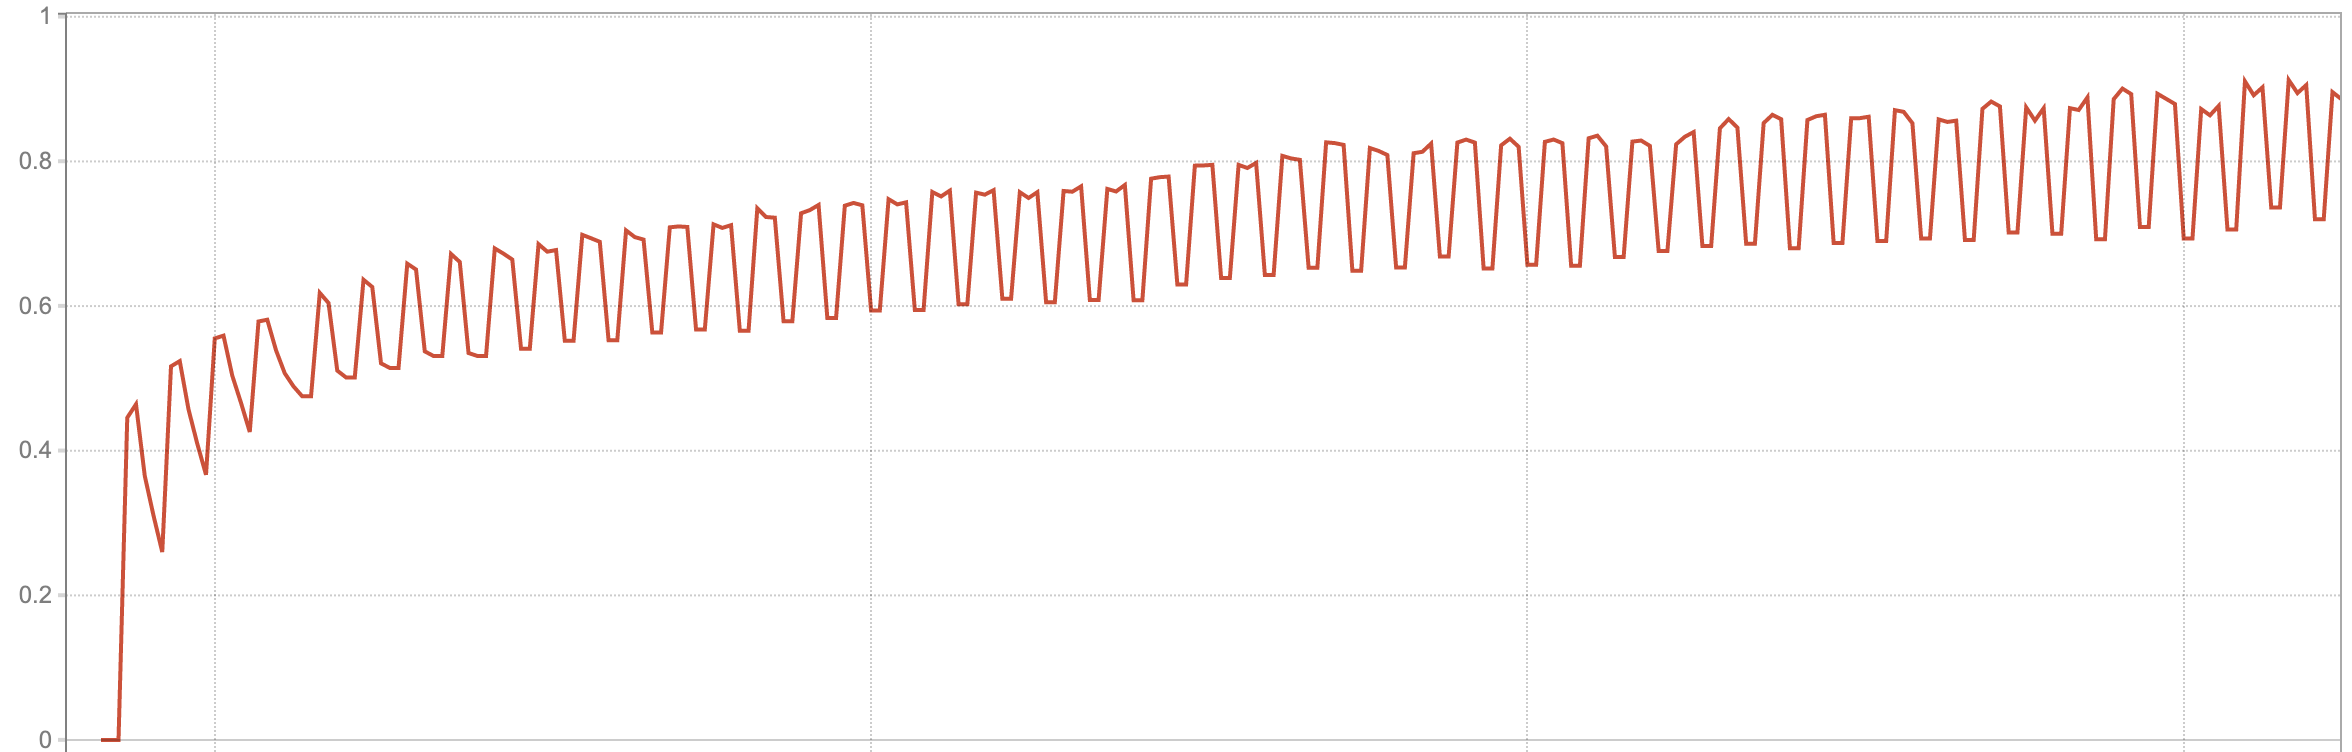
\includegraphics[width=\textwidth]{gfx/traffic_network_accuracy}
    \caption{Network traffic accuracy}
    \label{fig:network_traffic_accuracy}
\end{figure}

\begin{table}[ht]
    \centering
    \begin{tabular}{r|rrr|r}
        \multirow{2}{*}{K-value} & \multicolumn{3}{|c|}{Accuracy} & \multirow{2}{*}{CPU Usage} \\
        & Min & Max & average & \\ \hline        
        0 & 0.53& 1.22& 1.10& 9\% \\
        3 & 0.52& 1.04& 1.00& 4\% \\
        6 & 0.95& 1.74& 1.66& 3\% \\
        9 & 0.53& 1.29& 1.05& 3\% \\
        12& 0.93& 1.33& 1.10& 2\% \\
        15& 0.51& 1.11& 1.01& 2\% \\        
    \end{tabular}
    \caption{Network traffic accuracy results for different K-values}
    \label{tab:accuracy_results}
\end{table}

